%----------------------------------------
\subsection{Stencil Kernels}
\label{sect:stencil}
%----------------------------------------
To numerically solve a set of PDEs, iterative methods (finite difference, finite volume, finite element methods etc.) are frequently used to approximate the solution through a discretized (step by step) process. Thus, the continuous time and space domains are discretized so that a set of numerical computations are iteratively (time discretization) applied onto a mesh (space discretization). In other words, in a mesh-based numerical simulation, the PDEs are transformed to a set of numerical computations applied at each time step on elements of the discretized space domain (the mesh).
This paper focuses on one specific category of such numerical schemes based on \textit{stencil kernels}~\cite{spaaTangCKLL11}, also called in applied mathematics explicit numerical schemes.
This section introduces some definitions related to stencil kernels.

A \emph{mesh} is the discretization of a physical domain. It is a connected undirected graph without bridges (an edge is a bridge if its removal results in two disconnected graphs), where nodes and edges are linked to form cells (closure). Most of the time, nodes of a mesh are linked to coordinates in the real space domain. An example of structured mesh is illustrated in Figure~\ref{fig:mesh}. Each cell contains four nodes and four edges. \emph{Mesh entities} are elements of the mesh, such as the center of cells, edges or nodes. In Figure~\ref{fig:mesh}, two mesh entities are illustrated, the center of the cells (named \texttt{Cells}, in red) and edges on the horizontal axis (named \texttt{Edgex}, in blue on left and right of each cell). A \emph{data} is a simulated quantity on which computations are performed. Each data is mapped onto mesh entities. For example, in Figure~\ref{fig:ex1}, data $A$ and $B$ are mapped onto the center of cells, while, in Figure~\ref{fig:ex2}, $C$ is mapped onto the edges.
%\todo[inline]{JB: structured/unstructured pas defini, pas de notion de coordonees des elements du maillage dans l'espace reel?}


\begin{figure}
\begin{center}
\subfloat[Mesh and mesh domains.\label{fig:mesh}]{
\resizebox{7cm}{!}{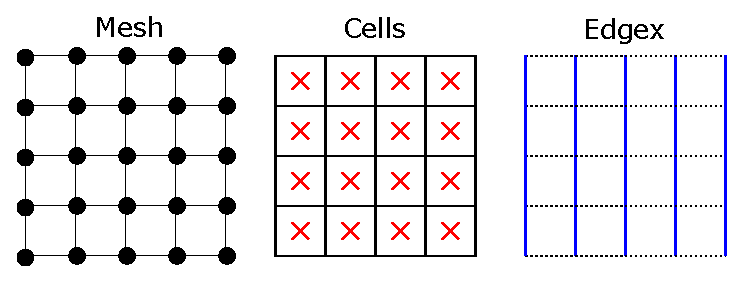
\includegraphics{./images/mesh.pdf}}
}
\hspace{10pt}
\subfloat[4-neighborhood stencil.\label{fig:ex1}]{
\resizebox{5cm}{!}{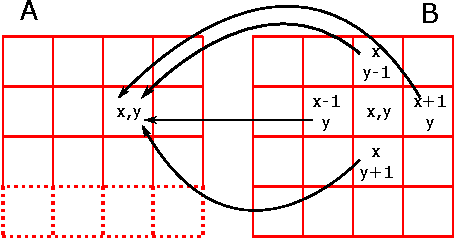
\includegraphics{./images/stencil1.pdf}}
}
\hspace{10pt}
\subfloat[2-neighborhood 2-entity stencil.\label{fig:ex2}]{
\resizebox{5cm}{!}{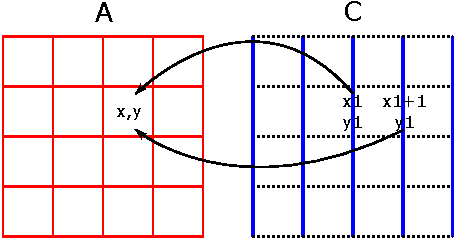
\includegraphics{./images/stencil2.pdf}}
}
\end{center}
\caption{(a) a Cartesian mesh and two kind of mesh entities, (b) an example of stencil kernel on cells, (c) an example of stencil kernel on two different entities of the mesh.}
\label{fig:gspmsp}
\end{figure}

% \begin{figure}[!h]\begin{center}
%   \resizebox{7cm}{!}{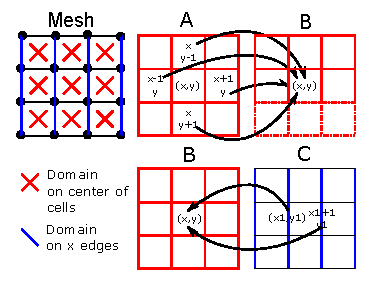
\includegraphics{./images/stencil.pdf}}
%   \caption{Examples of a stencil computations}
%   \label{fig:ex}
% \end{center}\end{figure}

A \emph{stencil kernel} computes the value of one data or a subpart of it (the kernel \emph{computation domain}) using a \emph{numerical expression} which takes as input one or more data.
For example, the stencil kernel illustrated in Figure~\ref{fig:ex1} computes $A$ using $B$, while the one in Figure~\ref{fig:ex2} computes $A$ using $C$. Thus, a stencil kernel is defined by its numerical expression, a set of input data (only one in the examples), and its unique output data, the result. 
The \emph{computation domain} is a subset of the mesh entities on which the output data is mapped. For example, in the first stencil, the computation of $A$ is performed on elements represented with full lines, while dotted elements are not computed. On the other hand, on the second computation, the computation domain of $A$ contains all the mesh entities on which it is mapped. This computation domain defines the elements over which the space loop iterates.

The numerical expression of a stencil kernel has the particularity to compute each element of the result independently using some elements of the inputs in a given neighborhood.
Accessed elements form a \emph{neighborhood} of the output known as the \emph{stencil shape}. For example, the stencil shape of the first computation in Figure~\ref{fig:ex1} contains direct neighbors on the right, left, top and bottom. Sometimes, the neighborhood can also access different mesh entities, as for example in Figure~\ref{fig:ex2}. Actually, in this computation, the neighborhood contains edges on the left and on the right of a cell. As an example, the numerical expression of the first example could be:
\begin{equation*} 
A(x,y) = B(x+1,y)+B(x-1,y)+B(x,y+1)+B(x,y-1),
\end{equation*}
and the numerical expression of the second kernel could be:
\begin{equation*} 
A(x,y) = A(x,y)+C(x1,y1)+C(x1+1,y1).
\end{equation*}

As it can be seen from these definitions, stencil kernels implementations share many properties from an algorithmic point of view that can be used to apply well known optimization and parallelization strategies.
Many solutions (languages or frameworks) thus propose to ease their programming by producing optimized and parallelized code from a simple description of the local computation to apply on each element.
These are further discussed in Sections~\ref{sect:related}.

%To resume, concepts used in this paper to define a stencil kernel are \emph{mesh}, \emph{mesh entities}, \emph{data}, \emph{computation domain}, \emph{numerical expression} and \emph{stencil shape}. 
While stencil kernels have been studied a lot, the formalization of real overall mesh-based numerical simulations is poorly studied and not exactly for the same kind of appication~\cite{Ragan-Kelley:2013:HLC:2491956.2462176}. Actually, paying attention to complex numerical simulations, it appears that most of them are composed of more than one stencil kernel, with one or more stencil shapes and of additional local computations. For example, we would like to formalize and parallelize a numerical simulation which chains the stencil kernels of Figures~\ref{fig:ex1} and~\ref{fig:ex2}. The next section formalizes concepts of \emph{stencil kernel}, \emph{local kernel} and \emph{multi-stencil program}.

%----------------------------------------
\subsection{A Multi-Stencil Formalization}
\label{sect:multistencil}
%----------------------------------------
This section introduces some formal definitions used in the rest of the paper.
Let $\Delta$ be the set of data of the simulation
A stencil kernel $s$ is defined as the quadruplet:
\begin{equation} 
s(R,w,exp,d),
\label{eq:st}
\end{equation}
where $R$ is a set of pairs $(r,n)$, with $r \in \Delta$ a data read by the computation, and $n$ the stencil shape (neighborhood) used to access $r$. The data written by the kernel is denoted $w \in \Delta$. $exp$ is the numerical expression of the stencil kernel. Finally the numerical expression is applied on the computation domain $d$.

For example, in Figure~\ref{fig:ex1}, assuming the computation domain (full lines) is $dc1$ and the stencil shape is $n1$, the stencil kernel can be defined as:
\begin{equation*}
R: \{(B,n1)\}, \quad w: A, \quad d: dc1,
\end{equation*}
\begin{equation*}
exp: A(x,y)=B(x+1,y)+B(x-1,y)+B(x,y+1)+B(x,y-1).
\end{equation*}
On the other hand, in the example of Figure~\ref{fig:ex2}, assuming the computation domain is $dc2$ and the stencil shape is $n2$, the stencil kernel is defined as:
\begin{equation*}
R: \{(C,n2),(A,local)\}, \quad w: A, \quad d: dc2,
\end{equation*}
\begin{equation*}
exp: A(x,y)=A(x,y)+C(x1,y1)+C(x1+1,y1).
\end{equation*}
One can notice that the input data $A$ is associated to the stencil shape $local$. This means that the stencil shape applied on $A$ is limited to the element with the exact same coordinate as the result element.

The specificities of kernels whose stencil shapes are all local makes it possible to apply specific optimizations.
We therefore provide a specific definition in this case.
A local (or auxiliary) kernel $l$ is defined as the quadruplet:
\begin{equation} 
l(R_l,w,exp,d),
\label{eq:loc}
\end{equation}
where $R_l$ is the set of input data locally accessed, and other parameters are the same as for normal stencil kernels.

We define a multi-stencil program as a sextuplet:
\begin{equation} 
\mathcal{MSP}(T,\mathcal{M},\mathcal{E},\mathcal{D},\Delta,\Gamma),
\label{eq:msp}
\end{equation}
where $T$ is the set of time iteration to run the simulation, $\mathcal{M}$ is the mesh of the simulation, $\mathcal{E}$ is the set of mesh entities, $\mathcal{D}$ is the set of computation domains used for computations, $\Delta$ is the set of data of the simulation, each one mapped onto a mesh entity, and finally $\Gamma$ is the set of computations. The set of computations $\Gamma$ is an ordered list of stencil and local kernels.
One can notice that this work, for now, is limited to a single mesh type for a given simulation.

% !!!!!!!!!!!! a mettre en plus court autre part !!!!!!!!!!!!!!!
%----------------------------------------
% \subsection{Parallelization techniques}
% \label{sect:parallel}
%----------------------------------------
% Three classical parallelization techniques are used in this paper and are described in this section, the data parallelism, the task parallelism, and the hybrid data and task parallelism. Those parallelization techniques are independent from the actual parallel hardware used.

% \paragraph{Data parallelism} The idea of this parallelization technique is to split, or partition, data on which computations are applied among available processors (or cores). Each processor then applies the same progam or instruction onto its subpart of data. Moreover, if a neighborhood information is needed from another processor communications or synchronizations are performed. 

% In the domain of numerical simulations, this technique is most of the time called a domain decomposition. This parallelization technique produce efficient programs up to thousands processors or cores, but on certain conditions. First, each subpart of data has to be big enough to overlap communication time. Second, the partitioning of data has to be balanced among processors. Thus, if this parallelization technique is clearly adequate to structured meshes, easy to balance, it is not for unstructured meshes or irregular structures where the amount of work is not heterogenous.

% \paragraph{Task parallelism} Another well known parallelization technique is to identify in a program the different tasks and which one are independant and can be launched concurrently. Most of the time, such a prallelization technique create a dependency directed acyclic graph (dependency dag) from a set of ordered tasks. Dependencies are found from read/write information for each task. Actually, if a task $i$ write a data $a$ and if a task $j$ read $a$, then $i$ has to be finished before $j$ is performed. From a dependency graph two different solutions are available. First, a static schedule of tasks is built, which could be a good solution if the tasks are regular, or use a dynamic scheduler to dynamically decide at runtime which task is executed on which processor.

% \paragraph{Hybrid parallelism} Finally, it is also possible to combine both those parallelization techniques to get what is called an hybrid parallelization. The interest of an hybrid parallelization is to bring another source of parallelism if limits of a given technique are reach.

